\documentclass[tikz,border=5pt]{standalone}
\usepackage{tikz}
\usetikzlibrary{shapes,arrows.meta,positioning,fit}

\definecolor{kernel}{HTML}{EAF7EA}
\definecolor{surface}{HTML}{E9F2FF}
\definecolor{textgray}{HTML}{444444}

\tikzset{
  category/.style={
    draw=textgray,
    rounded corners=4pt,
    fill=surface,
    align=center,
    minimum width=32mm,
    minimum height=12mm,
    font=\sffamily\small,
    very thick
  },
  core/.style={
    draw=textgray,
    rounded corners=6pt,
    fill=kernel,
    align=center,
    minimum width=40mm,
    minimum height=14mm,
    font=\sffamily\normalsize\bfseries,
    very thick
  },
  arrow/.style={
    -{Latex[length=3mm,width=2mm]},
    very thick,
    draw=textgray
  }
}

\begin{document}
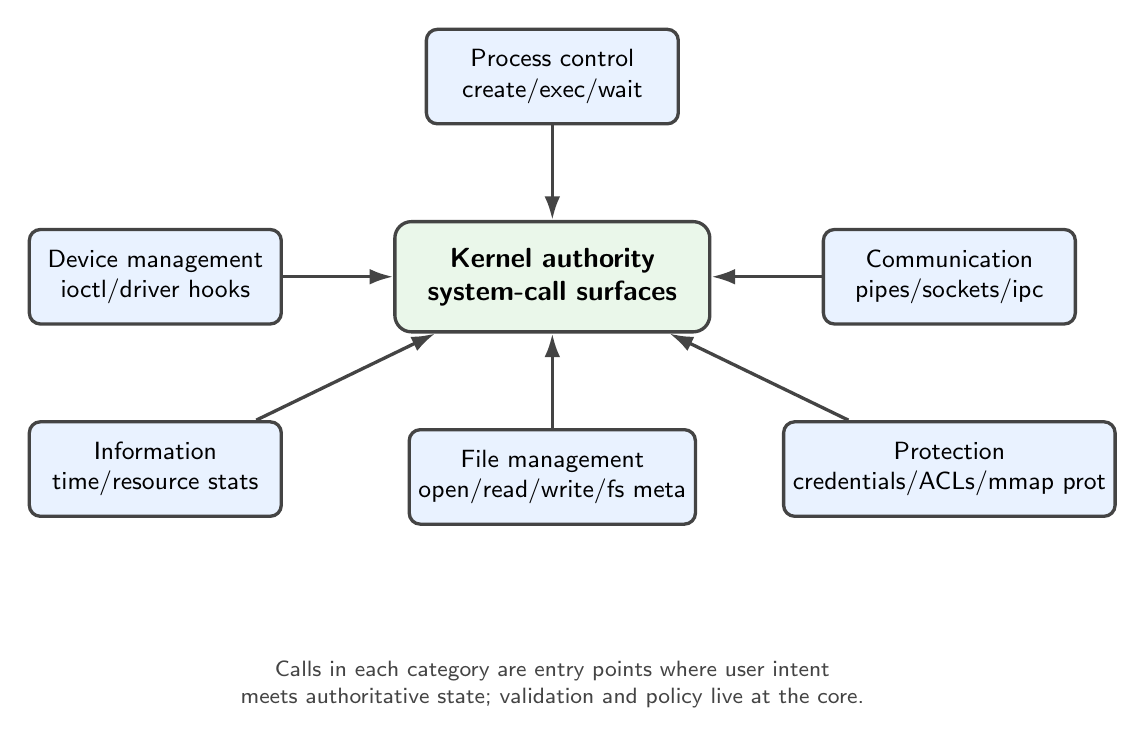
\begin{tikzpicture}[node distance=12mm and 14mm]
  \node[core] (core) {Kernel authority\\system-call surfaces};

  \node[category, above=of core] (proc) {Process control\\create/exec/wait};
  \node[category, below=of core] (file) {File management\\open/read/write/fs meta};
  \node[category, left=of core] (device) {Device management\\ioctl/driver hooks};
  \node[category, right=of core] (comm) {Communication\\pipes/sockets/ipc};

  \node[category, below=of device] (info) {Information\\time/resource stats};
  \node[category, below=of comm] (protect) {Protection\\credentials/ACLs/mmap prot};

  \draw[arrow] (proc) -- (core);
  \draw[arrow] (device) -- (core);
  \draw[arrow] (file) -- (core);
  \draw[arrow] (comm) -- (core);
  \draw[arrow] (info) -- (core);
  \draw[arrow] (protect) -- (core);

  \node[draw=none, align=center, font=\sffamily\footnotesize, text=textgray, below=16mm of file]
    (note) {Calls in each category are entry points where user intent\\
    meets authoritative state; validation and policy live at the core.};
\end{tikzpicture}
\end{document}
